\section{Segmentation task}
The last number of the Enric's ID card is the 46. Since the division of 46 by 6 has a 
remainder of 4, it will be used the fourth option of data that is a segmentation of the 
lungs along with the major thoracic bones. To do it the data will be downloaded from the 
Download sample data option in the Welcome to slicer module. The data choose is the CTCchest.


The first step to segmentate the pulmons is to add a segment for it. It is called “Pulmons” 
and it  has been selected as a dark red color that usually is used for the organs of the body. 
The segmentation of the organ is done by different modes of segmentation:

\subsection{Threshold segmentation}
This is the most basic and most widely used segmentation technique in medical images. 
The technique is based on the set of a threshold value for the intensity of each  pixel 
in the image. All those pixels that are in the range of the threshold value will be shown 
at the same time that all the pixels that are not in the range will not be shown. It is a 
kind of binari tool to differentiate types of pixels.\\
To set the threshold value in the slicer program it is used a tool that allows you to select 
the organ's zone that you want to see by a cerquel in the image. In \textbf{\textit{\cref{fig:threshold_tool}}}. it can be seen 
the usage of the selection tool to select a part of the pulmons.

\begin{figure}[H]
    \centering
    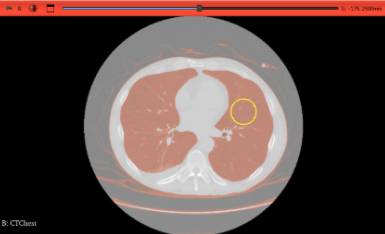
\includegraphics[width=0.7\textwidth]{img/ex1_1.png}
    \caption{Visualitzation of the selected zone of the lungs to set the threshold value.}
    \label{fig:threshold_tool}
\end{figure}

With this tool it has been set a threshold range between the 
values of (-931 , -343) that all the pixels of the lung share.
The 3D visualization using just this technique is the one that 
is shown in the \textbf{\textit{\cref{fig:threshold_tool}}}.

\begin{figure}[H]
    \centering
    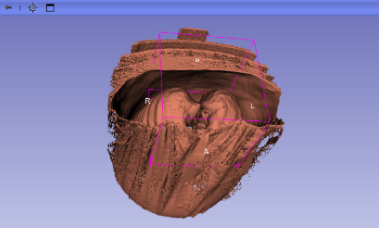
\includegraphics[width=0.7\textwidth]{img/ex1_2.png}
    \caption{visualization of the result of the threshold segmentation tool on the CTChest model.}
    \label{fig:threshold_result}
\end{figure}


By looking at the results of the first segmentation it is clear 
that  the pulmons pixels are in the threshold range but also a lot
of non important body data is on that range so it needs to be 
eliminated from the visualitzation to see clearly the organ. 
To do it there are other segmentation techniques that are useful. 

\subsection{Scissors segmentation}
The segmentation scissors tool is a good technique to clean our image from undesired data. By using the scissors tool that is on the left part of the program screen can be selected the wrong data of the image by circling it in a plane, as it is seen in \textbf{\textit{\cref{fig:scissors_tool}}}.

\begin{figure}[H]
    \centering
    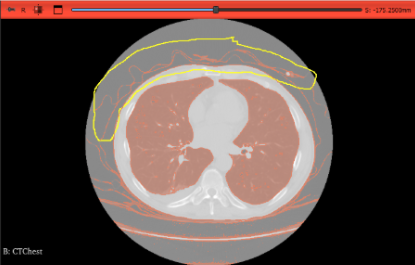
\includegraphics[width=0.7\textwidth]{img/ex13.png}
    \caption{Usage of the scissors segmentation tool on the upper vision of the lungs to eliminate data that is not from our interest.}
    \label{fig:scissors_tool}
\end{figure}

This technique allows us to erase all the undesired data of the image, in the \textbf{\textit{\cref{fig:scissors_tool}}} can be seen our model once this technique is used on it.

\begin{figure}[H]
    \centering
    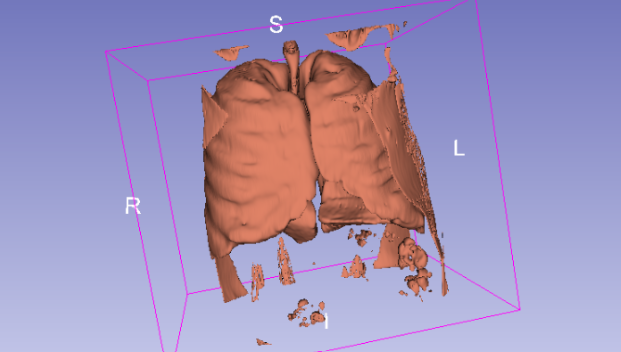
\includegraphics[width=0.7\textwidth]{img/ex14.png}
    \caption{Results of the scissor segmentation tool usage on the CTChest mode.}
    \label{fig:scissors_result}
\end{figure}


\subsection{Islands segmentation}
Another technique to edit the segmentation is the called islands. In the left column of the slicer program can be selected the island tool and by selecting the rest of the pixels that are not from the lungs they can be erased from the image as it is shown in the \textbf{\textit{\cref{fig:islands_tool}}}.

\begin{figure}[H]
    \centering
    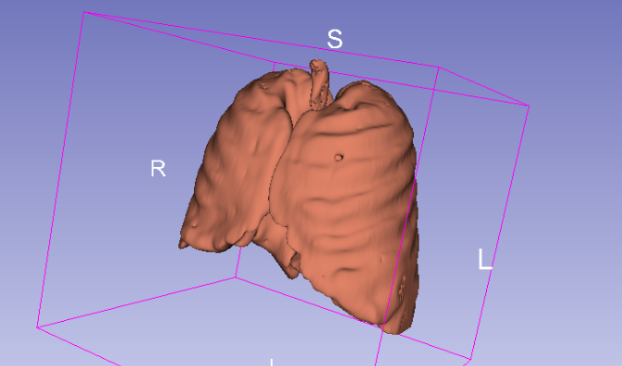
\includegraphics[width=0.7\textwidth]{img/ex15.png}
    \caption{Visual result of island tool usage on the CTChest model.}
    \label{fig:islands_tool}
\end{figure}

The objective of the exercise is to visualize the lungs and the thoracic bones so to do it another segmentation is created called “Major thoracic bones”. Another threshold range is created with the values of (85, 463). The results are shown in the \textbf{\textit{\cref{fig:thoracic_bones}}}.

\begin{figure}[H]
    \centering
    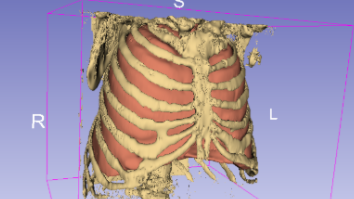
\includegraphics[width=0.7\textwidth]{img/ex16.png}
    \caption{Visual result of the thoracic bones segmentation on the CTChest model.}
    \label{fig:thoracic_bones}
\end{figure}

By using the scissors and the islands techniques explained before the image is processed to discard the visualization of the pixels that are not interesting for this visualization. The result is shown in the \textbf{\textit{\cref{fig:final_result}}}.

\begin{figure}[H]
    \centering
    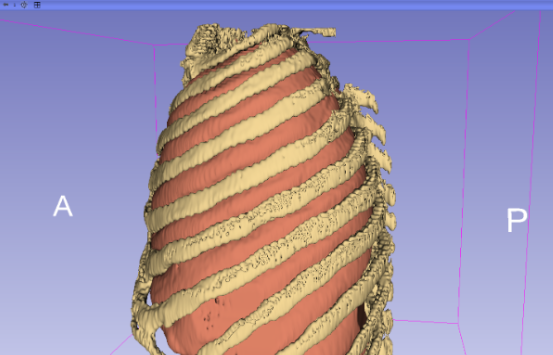
\includegraphics[width=0.7\textwidth]{img/ex17.png}
    \caption{Lateral vision of the scissor tool usage on the CTChest model to eliminate the bones parts are not from the torcic bones. This is the final segmentation result of the exercise.}
    \label{fig:final_result}
\end{figure}

